% !TEX encoding = UTF-8 Unicode
%%%%%%%%%%%%%%%%%%%%%%%%%%%%%%%%%%%%%%%%%
% Beamer Presentation
% LaTeX Template
% Version 1.0 (10/11/12)
%
% This template has been downloaded from:
% http://www.LaTeXTemplates.com
%
% License:
% CC BY-NC-SA 3.0 (http://creativecommons.org/licenses/by-nc-sa/3.0/)
%
%%%%%%%%%%%%%%%%%%%%%%%%%%%%%%%%%%%%%%%%%

%----------------------------------------------------------------------------------------
%	PACKAGES AND THEMES
%----------------------------------------------------------------------------------------

\documentclass{beamer}

\mode<presentation> {

% The Beamer class comes with a number of default slide themes
% which change the colors and layouts of slides. Below this is a list
% of all the themes, uncomment each in turn to see what they look like.

%\usetheme{default}
%\usetheme{AnnArbor}
%\usetheme{Antibes}
%\usetheme{Bergen}
%\usetheme{Berkeley}
%\usetheme{Berlin}
%\usetheme{Boadilla}
%\usetheme{CambridgeUS}
%\usetheme{Copenhagen}
%\usetheme{Darmstadt}
%\usetheme{Dresden}
%\usetheme{Frankfurt}
%\usetheme{Goettingen}
%\usetheme{Hannover}
%\usetheme{Ilmenau}
%\usetheme{JuanLesPins}
%\usetheme{Luebeck}
%\usetheme{Madrid}
%\usetheme{Malmoe}
%\usetheme{Marburg}
%\usetheme{Montpellier}
%\usetheme{PaloAlto}
%\usetheme{Pittsburgh}
%\usetheme{Rochester}
\usetheme{Singapore}
%\usetheme{Szeged}
%\usetheme{Warsaw}

% As well as themes, the Beamer class has a number of color themes
% for any slide theme. Uncomment each of these in turn to see how it
% changes the colors of your current slide theme.

%\usecolortheme{albatross}
%\usecolortheme{beaver}
%\usecolortheme{beetle}
%\usecolortheme{crane}
%\usecolortheme{dolphin}
%\usecolortheme{dove}
%\usecolortheme{fly}
%\usecolortheme{lily}
%\usecolortheme{orchid}
%\usecolortheme{rose}
%\usecolortheme{seagull}
%\usecolortheme{seahorse}
%\usecolortheme{whale}
%\usecolortheme{wolverine}

%\setbeamertemplate{footline} % To remove the footer line in all slides uncomment this line
%\setbeamertemplate{footline}[page number] % To replace the footer line in all slides with a simple slide count uncomment this line

%\setbeamertemplate{navigation symbols}{} % To remove the navigation symbols from the bottom of all slides uncomment this line
}

\usepackage{graphicx} % Allows including images
\usepackage{booktabs} % Allows the use of \toprule, \midrule and \bottomrule in tables
\usepackage{xeCJK}
\setCJKmainfont{SourceHanSerif-Regular}
\usepackage{color}
\usepackage{listings}
\lstset{numbers=left}
\usepackage{tikz}


%----------------------------------------------------------------------------------------
%	TITLE PAGE
%----------------------------------------------------------------------------------------

\title[Django]{Django} % The short title appears at the bottom of every slide, the full title is only on the title page
\subtitle{Introduce}
\author{} % Your name
\institute[计算机科学与技术学院] % Your institution as it will appear on the bottom of every slide, may be shorthand to save space
{
贵州大学 \\ % Your institution for the title page
\medskip
\textit{hnzhang1@gzu.edu.cn} % Your email address
}
\date{\today} % Date, can be changed to a custom date

\begin{document}

\begin{frame}
\titlepage % Print the title page as the first slide
\end{frame}
\begin{frame}{Overview}
\tableofcontents
\end{frame}
\section{Introduction}
\begin{frame}{github repository of python web framworks (2018.12.24)}
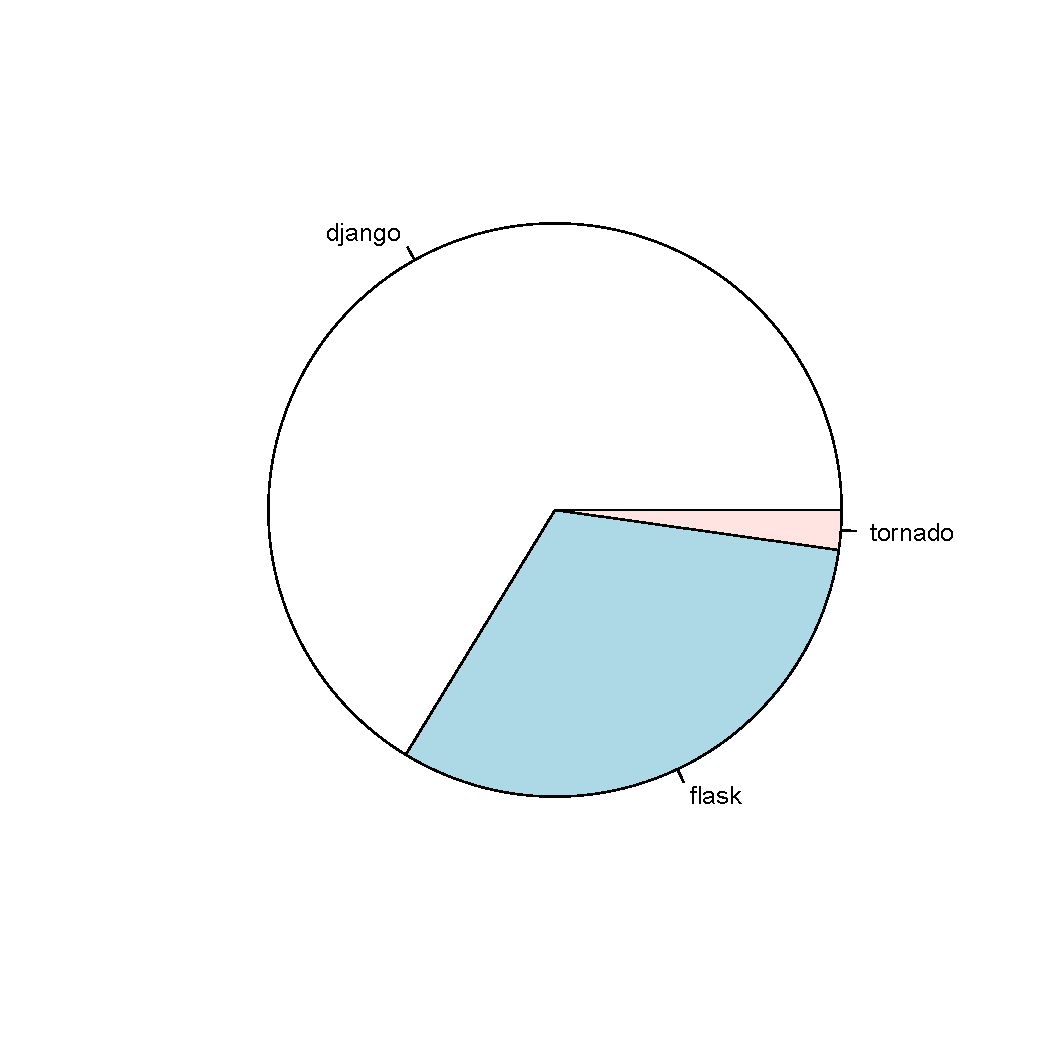
\includegraphics[height=1\textheight]{django-introduce-1.pdf}
\end{frame}
\begin{frame}{django}
Django is a high-level \textcolor{red}{Python Web framework} that encourages rapid development and clean, pragmatic design. Built by experienced developers, it takes care of much of the hassle of Web development, so you can focus on writing your app without needing to \textcolor{blue}{reinvent the wheel}. It’s free and open source. 
\end{frame}
\begin{frame}{Django features}
% \begin{block}
 \begin{itemize}
 \item ridiculously fast
 \item fully loaded
 
 Django includes dozens of extras you can use to handle common Web development tasks. Django takes care of user authentication, content administration, site maps, RSS feeds, and many more tasks — right out of the box.
 \item reassuringly secure
 
 Django includes dozens of extras you can use to handle common Web development tasks. Django takes care of user authentication, content administration, site maps, RSS feeds, and many more tasks — right out of the box.
 \item exceedingly scalable
 \item incredibly versatile
 
 Companies, organizations and governments have used Django to build all sorts of things — from content management systems to social networks to scientific computing platforms.
 \end{itemize}
% \end{block}
\end{frame}
\begin{frame}{install}
\begin{itemize}
\item quick install guide\footnote{Python includes a lightweight database called SQLite so you won’t need to set up a database just yet. Django includes a lightweight web server you can use for testing, so you won’t need to set up Apache until you’re ready to deploy Django in production.}

\url{https://docs.djangoproject.com/en/2.1/intro/install/}
\item complete installation guide

\url{https://docs.djangoproject.com/en/2.1/topics/install/}
\end{itemize}
\end{frame}
\begin{frame}[fragile]{quick install guide}
\begin{enumerate}
\item install python 3.7
\item install Django
\begin{enumerate}
\item install pip3
\item pip3 install django
\end{enumerate}
\item verifying
\begin{verbatim}
$ python3
Python 3.7.0 (v3.7.0:1bf9cc5093, Jun 26 2018, 23:26:24) 
[Clang 6.0 (clang-600.0.57)] on darwin
Type "help", "copyright", "credits" or "license" for more information.
>>> import django
>>> print(django.get_version())
2.1.4
>>> 

\end{verbatim}
\end{enumerate}
\end{frame}
\begin{frame}[fragile]{create a project}
From the command line, cd into a directory where you’d like to store your code, then run the following command:
\begin{verbatim}
$ pwd
/Users/hainingzhang/Documents/GitHub/dm-web/web
$ django-admin startproject mysite
$ tree
.
|____mysite
| |____mysite
| | |______init__.py
| | |____settings.py
| | |____urls.py
| | |____wsgi.py
| |____manage.py

\end{verbatim}
\end{frame}
\begin{frame}[fragile]{runserver}
Let’s verify our Django project works. Change into the outer mysite directory, and run the following commands:
\begin{verbatim}
$ python3 manage.py runserver
Performing system checks...
…
December 24, 2018 - 11:37:11
Django version 2.1.4, using settings 'mysite.settings'
Starting development server at http://127.0.0.1:8000/
Quit the server with CONTROL-C.
\end{verbatim}
Now that the server’s running, visit http://127.0.0.1:8000/ with your Web browser. You’ll see a “Congratulations!” page, with a rocket taking off. It worked!\footnote{don’t use this server in anything resembling a production environment. At the same time a new file db.sqlite3 is created.}
\end{frame}
\begin{frame}{project files}
\begin{itemize}
\item the outer mysite/ root directory is just a container for your project. 
\item manage.py: A command-line utility that lets you interact with this Django project in various ways. 
\item the inner mysite/ directory

 is the actual Python package for your project. Its name is the Python package name you’ll need to use to import anything inside it (e.g. mysite.urls).
\item \_\_init\_\_.py: An empty file that tells Python that this directory should be considered a Python package. 
\item settings.py: Settings/configuration for this Django project. 
\item urls.py: The URL declarations for this Django project; a “table of contents” of your Django-powered site. 
\item wsgi.py: An entry-point for WSGI-compatible web servers to serve your project. 
\end{itemize}
\end{frame}
\begin{frame}[fragile]{crate an app}
Our environment – a “project” – is set up, we’re set to start doing work.
To create our app, make sure you’re in the same directory as manage.py and type this command:
\begin{verbatim}
$ python3 manage.py startapp blog
\end{verbatim}
\end{frame}
\begin{frame}[fragile]{app structure}
\begin{verbatim}
|____mysite
| |______init__.py
| |______pycache__
| |____settings.py
| |____urls.py
| |____wsgi.py
|____db.sqlite3
|____blog
| |____migrations
| |____models.py
| |______init__.py
| |____apps.py
| |____admin.py
| |____tests.py
| |____views.py
|____manage.py
\end{verbatim}
\end{frame}
\begin{frame}{projects vs. apps}
What’s the difference between a project and an app? An app is a Web application that does something – e.g., a Weblog system, a database of public records or a simple poll app. A project is a collection of configuration and apps for a particular website. A project can contain multiple apps. An app can be in multiple projects.
\end{frame}
\section{write the app: blog}
\begin{frame}{creating models}
A model is the single, definitive source of truth about your data. It contains the essential fields and behaviors of the data you’re storing. (\textcolor{red}{like a table in the database})

Edit the blog/models.py file:
\end{frame}
%----------------------------------------------------------------------------------------
%	PRESENTATION SLIDES
%----------------------------------------------------------------------------------------
\section{Q\&A}
\begin{frame}
\center{\Huge{Q\&A}}
\end{frame}

%How do I uninstall?
%
%	1.	Remove /Applications/Wireshark.app
%	2.	Remove /Library/Application Support/Wireshark
%	3.	Remove the wrapper scripts from /usr/local/bin
%	4.	Unload the org.wireshark.ChmodBPF.plist launchd job
%	5.	Remove /Library/LaunchDaemons/org.wireshark.ChmodBPF.plist
%	6.	Remove the access_bpf group.
%	7.	Remove /etc/paths.d/Wireshark
%	8.	Remove /etc/manpaths.d/Wireshark
\end{document} 

